\documentclass[../../main.tex]{subfiles}

\graphicspath{{../../image/}{../../figure/}}

\begin{document}

\section{Transformer 语言模型}\label{section:ch12-Transformer语言模型}

Transformer 处理层是一个高度灵活的组件，可用于构建具有广泛适用性的强大神经网络模型。本节将探讨 Transformer 在自然语言中的应用。这促进了称作大语言模型（Large Language Model, LLM）的大规模神经网络的发展，事实证明，这类模型具有非凡的能力（Zhao et al., 2023）。

Transformer 语言模型可用于多种不同的语言处理任务，并可根据输入和输出数据的形式分为 3 类。在情感分析等问题中，我们将一个词序列作为输入，并提供一个代表文本情感（如快乐或悲伤）的变量作为输出。此处，Transformer 充当序列的“编码器”。而在其他问题中，我们可能会将单个向量作为输入，并生成一个词序列作为输出。例如，假设我们希望在给定输入图像的情况下生成文本标题。在这种情况下，Transformer 作为“解码器”产生一个序列作为输出。最后，在序列到序列的处理任务中，输入和输出都由一个词序列组成。例如，假设我们想要将一种语言翻译成另一种语言。在这种情况下，Transformer 同时扮演编码器和解码器的角色。我们将使用模型架构的说明性示例依次讨论上述每一类 Transformer 语言模型。

\subsection{解码器型 Transformer}\label{subsection:ch12-解码器型Transformer}

我们首先考虑解码器型 Transformer。此类 Transformer 语言模型可以用作生成式模型以创建 token 的输出序列。作为说明性示例，我们将重点讨论一种名为 GPT（Generative Pretrained Transformer，生成式预训练 Transformer）的模型（Radford et al., 2019; Brown et al., 2020; OpenAI, 2023）。我们想要利用 Transformer 架构构建一个形式如\eqref{align:ch12-自回归语言模型}的自回归模型，其中条件分布 $p(x_n\mid x_1,\cdots,x_{n-1})$ 是利用从数据中习得的 Transformer 神经网络来表示的。

该模型将由前 $n-1$ 个 token 组成的序列作为输入，相应的输出表示 token $n$ 的条件分布。从这个分布中抽取一个样本，即可将序列扩展到 $n$ 个 token，这个新序列可以通过模型反馈给 token $n+1$ 的分布，以此类推。可以重复该过程，生成一个序列，该序列的最大长度由 Transformer 输入的数量决定。我们稍后将讨论从条件分布中采样的策略（参见\cref{subsection:ch12-抽样策略}），但目前我们讨论的重点是如何构建和训练网络。

GPT 模型的架构由 Transformer 层堆叠组成，这些层采用 token 的序列 $\mathbf{x}_1,\cdots,\mathbf{x}_N$ 作为输入，维度为 $D$，并产生 token 的序列 $\tilde{\mathbf{x}}_1,\cdots,\tilde{\mathbf{x}}_N$ 作为输出，维度同样为 $D$。每个输出都需要代表该时间步的 token 字典的概率分布，token 字典的维度为 $K$，而 token 的维度为 $D$。因此，我们使用维度为 $D\times K$ 的矩阵 $\mathbf{W}^{(o)}$ 对每个输出 token 进行线性变换，然后使用 softmax 激活函数，其形式为
\begin{align}
\mathbf{Y}=\mathrm{Softmax}\left(\tilde{\mathbf{X}}\mathbf{W}^{(o)}\right)
\label{align:ch12-语言模型输出}
\end{align}

其中 $\mathbf{Y}$ 是第 $n$ 行为 $\mathbf{y}_n^{\mathsf{T}}$ 的矩阵，$\tilde{\mathbf{X}}$ 是第 $n$ 行为 $\tilde{\mathbf{x}}_n^{\mathsf{T}}$ 的矩阵。每个 softmax 输出单元都有一个相关的交叉熵误差函数（参见\cref{subsection:ch05-多类logistic回归}）。模型架构如\cref{figure:ch12-解码器GPT}所示。

\begin{figure}[htbp]
  \centering
  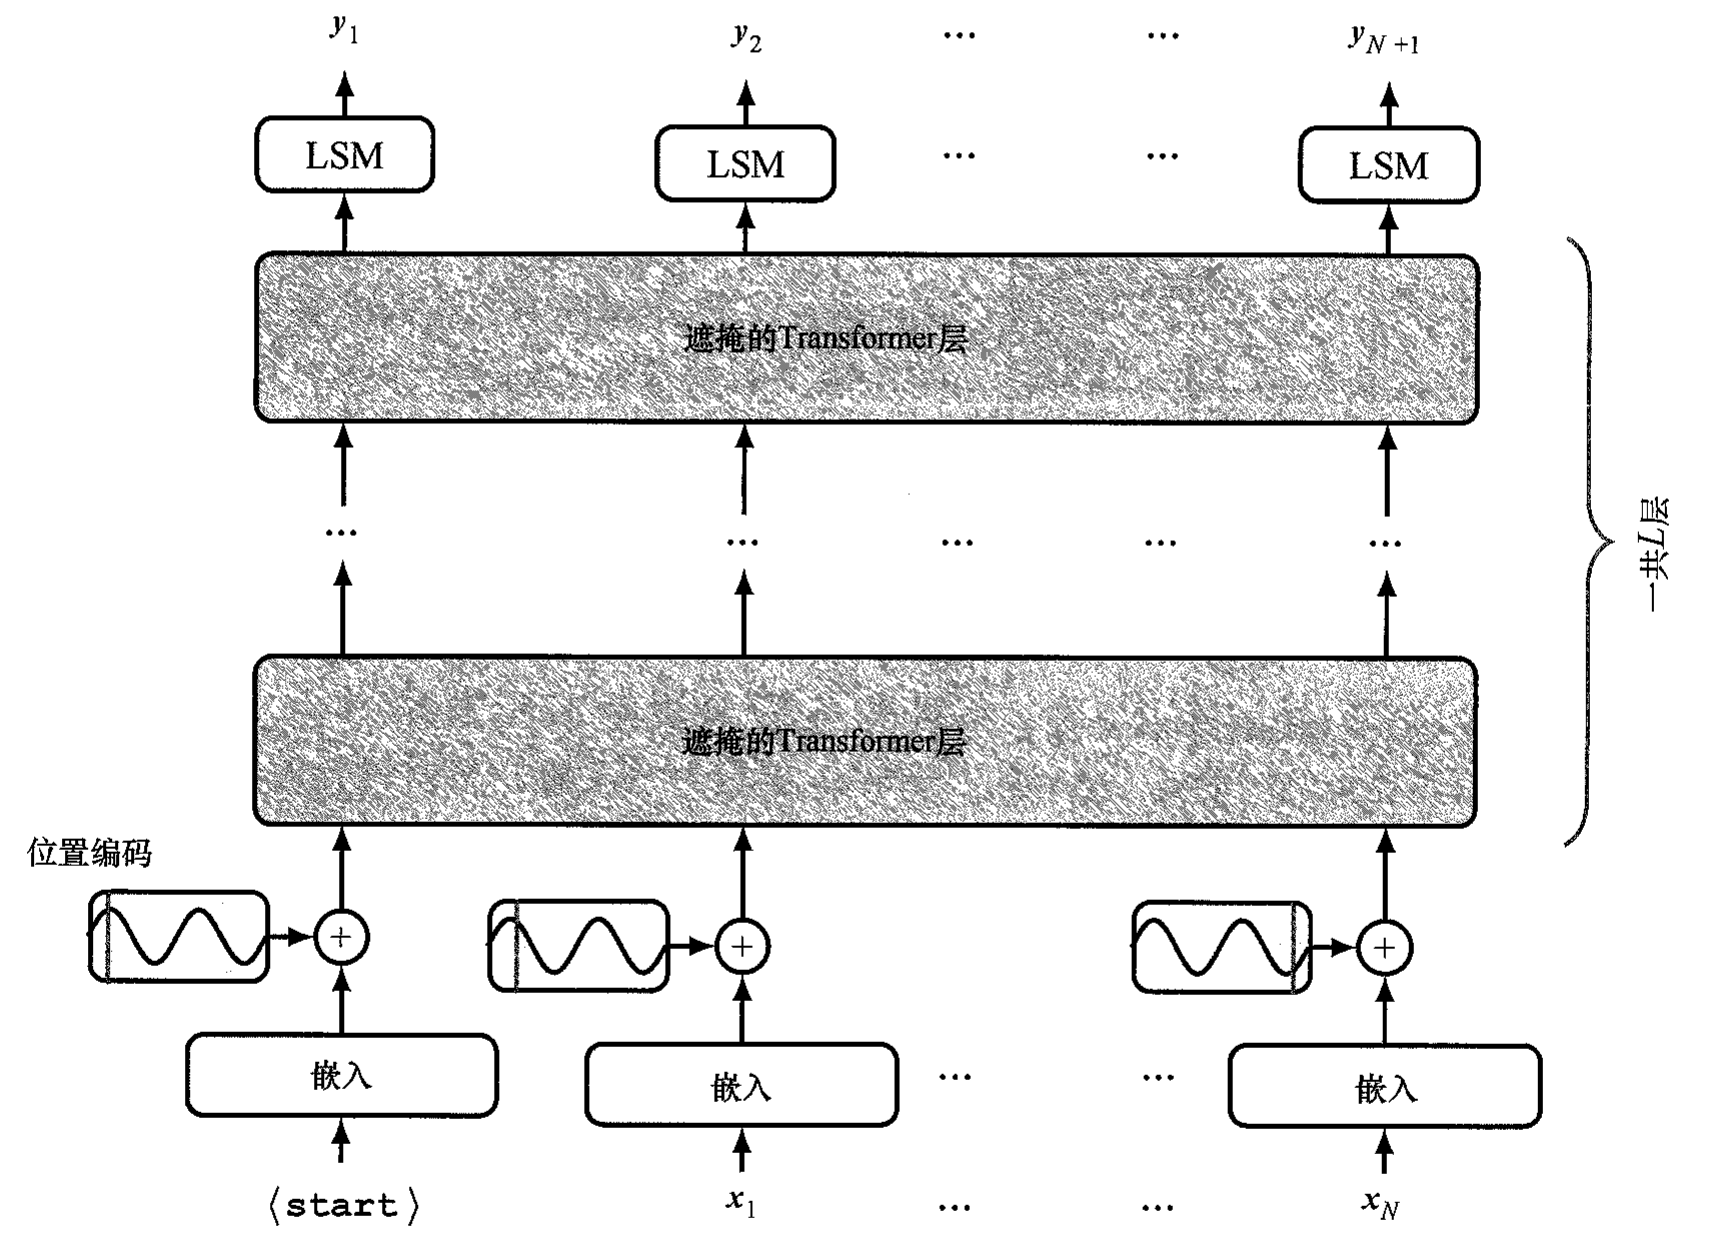
\includegraphics[width=0.8\textwidth]{ch12-fig12-15-decoder-gpt.png}
  \caption{GPT 解码器型 Transformer 网络的架构。此处“LSM”代表 linear-softmax，记作一种线性变换，它的可学习参数在 token 位置之间是共享的，然后是一个 softmax 激活函数。}
  \label{figure:ch12-解码器GPT}
\end{figure}

该模型可以采用自监督的方法并使用大规模的无标签自然语言语料进行训练。每个训练样本由 token 的序列 $\mathbf{x}_1,\cdots,\mathbf{x}_n$ 组成，构成网络的输入。每个训练样本还包含序列中下一个 token 组成的相关目标值 $\mathbf{x}_{n+1}$。序列可以认为是独立同分布的，因此用于训练的误差函数是训练集上的交叉熵误差值之和，并分成适当的小批次。我们可以使用通过模型的前向传递来独立且朴素地处理每个训练样本。不过，我们可以通过一次性处理整个序列来实现更高的效率，从而每个 token 既可以作为前一个 token 序列的目标值，也可以作为后续 token 的输入值。例如，考虑如下词序列：

\begin{center}
I swam across the river to get to the other bank.
\end{center}

我们既可以使用“I swam across”作为输入序列，关联目标为“the”；也可以使用“I swam across the”作为输入序列，关联目标为“river”，以此类推。不过，为了并行处理这些数据，我们必须确保网络无法通过提前查看序列来“作弊”，否则它只会学到将下一个输入直接复制到输出。这样的话，它就无法生成新的序列，因为根据定义，测试时后续 token 不可用。为了解决这个问题，我们做了两件事。首先，我们将输入序列向右移动一步，使输入 $\mathbf{x}_n$ 对应于输出 $\mathbf{y}_{n+1}$，目标为 $\mathbf{x}_{n+1}$，并在输入序列的第一个位置预置一个额外的 token，标记为 $\langle\mathrm{start}\rangle$。其次，请注意，Transformer 中的 token 是独立处理的，除非它们用于计算注意力权重，此时它们会通过点积成对地相互作用。因此，我们在每个注意层中引入了遮掩注意力（masked attention），有时也称因果注意力（causal attention）。在此过程中，我们将每个 token 对于序列中之后的所有 token 的注意力权重设为零。具体来说，只需要将\eqref{align:ch12-缩放点积注意力}定义的注意力矩阵 $\mathrm{Attention}(\mathbf{Q},\mathbf{K},\mathbf{V})$ 的所有相应元素置零，然后对其余元素进行归一化，使每一行的总和再次为 $1$ 即可。为达成这一目标，在实际操作中，可将相应的预激活值设置为 $-\infty$。这样一来，softmax 函数对相关输出的计算结果为零，并能对非零输出进行归一化处理。遮掩注意力矩阵的结构如\cref{figure:ch12-遮掩注意力}所示。

\begin{definition}[遮掩自注意力]\label{definition:ch12-遮掩自注意力}
设 $\mathbf{Q},\mathbf{K},\mathbf{V}$ 由\eqref{align:ch12-查询键值定义}给出。若对每个 $n$ 只允许位置 $m\leqslant n$ 的键参与注意力，即把 $m>n$ 的 softmax 预激活值置为 $-\infty$，其余按\eqref{align:ch12-缩放点积注意力}归一化，则称所得注意力为\textbf{遮掩自注意力}（masked self-attention）。
\end{definition}

% SUPPLEMENT: parent=definition:ch12-遮掩自注意力; kind=motivation; location=紧随其后的 remark（重构新增）
\begin{remark}（重构新增）
遮掩的作用是“在训练时模拟推理时的信息约束”：推理时位置 $n$ 只能看到前 $n$ 个 token，因此训练时也不许它看后面的内容，否则模型会退化为“复制下一个输入”的恒等映射。用 $-\infty$ 而不是 $0$ 来屏蔽是有讲究的：若把未归一化的权重置零，softmax 的分母仍包含这些项，归一化后每行之和不再是原先的 $1$，且被屏蔽项会分走概率质量；置 $-\infty$ 后 $\exp(-\infty)=0$，这些项在分子与分母中同时精确消失，归一化自动只在可见集合上进行。由于屏蔽模式只依赖位置而不依赖数据，它可以在每个注意力头、每一层复用同一张下三角掩码。定义中“$m\leqslant n$”包含自身，这是必要的：位置 $n$ 的表示必须能看见自己。
\end{remark}

\begin{figure}[htbp]
  \centering
  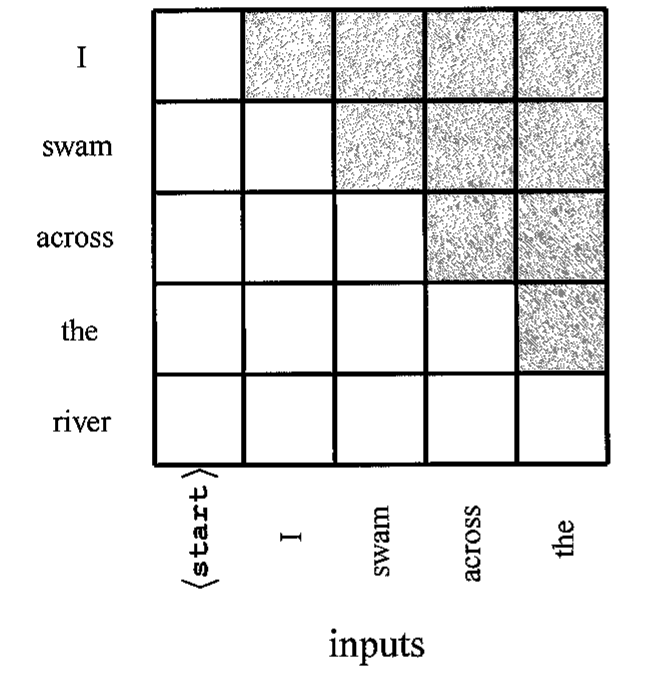
\includegraphics[width=0.36\textwidth]{ch12-fig12-16-masked-attention.png}
  \caption{遮掩注意力矩阵的结构。红色元素对应的注意力权重为零。因此，在预测 token“across”时，输出只能取决于输入 tokens“$\langle\mathrm{start}\rangle$”“I”和“swam”。}
  \label{figure:ch12-遮掩注意力}
\end{figure}

在实践中，我们希望有效利用 GPU 的大规模并行性，因此可以将多个序列堆叠成一个输入张量，以便在一个批次中进行并行处理。不过，这要求序列的长度相同，而文本序列的长度是可变的。要解决这个问题，我们可以引入一个特定的 token（用 $\langle\mathrm{pad}\rangle$ 表示），用来填充未使用的位置，从而使所有序列达到相同的长度，以便将它们合并成一个单一张量。然后在注意力权重中使用一个额外的掩码，以确保输出向量不对 $\langle\mathrm{pad}\rangle$ token 占用的任何输入给予注意力。请注意，该掩码的形式取决于特定的输入序列。

训练模型的输出是 token 空间的概率分布，其由输出激活函数 softmax 给出，表示当前 token 序列情况下的下一个 token 的概率。一旦选择了下一个词，就可以将包含新 token 的 token 序列再次输入模型，以生成序列中的后续 token，这个过程可以无限重复，直至生成表示序列结束的 token。这看起来似乎效率很低，因为每个新生成的 token 都必须通过整个模型输入数据。不过，请注意，由于遮掩注意力，为特定 token 所学习到的嵌入向量只取决于该 token 本身和先前的 token，因此在生成新的、后续的 token 时，该嵌入向量不会发生变化。在处理新的 token 时，大部分计算可以循环使用。

\subsection{抽样策略}\label{subsection:ch12-抽样策略}

我们已经看到，解码器型 Transformer 的输出是序列中下一个 token 值的概率分布，必须从中选择一个特定的 token 值来扩展序列。根据计算出的概率，选择 token 值的方法有好几种（Holtzman et al., 2019）。一种显而易见的方法称为贪婪搜索，即简单地选择概率最高的 token。这使得模型具有确定性，即给定的输入序列总是产生相同的输出序列。请注意，在每个阶段选择概率最高的 token 并不等于选择概率最高的 token 序列（见\cref{exercise:ch12-15}）。要找到最有可能的序列，我们需要最大化所有 token 的联合分布，其计算公式为
\begin{align}
p(\mathbf{y}_1,\cdots,\mathbf{y}_N)=\prod_{n=1}^{N}p(\mathbf{y}_n\mid\mathbf{y}_1,\cdots,\mathbf{y}_{n-1})
\label{align:ch12-序列联合分布}
\end{align}

如果序列中有 $N$ 个步骤，而字典中 token 值的数量为 $K$，那么序列的总数为 $O(K^{N})$，这使得序列的长度呈指数增长，因此寻找单一的最可能序列是不可行的。相比之下，贪婪搜索的成本为 $O(KN)$，与序列长度成线性关系。

与贪婪搜索相比，有一种技术有可能产生更高概率的序列，即束搜索（beam search）。我们不是在每一步都选择一个最可能的 token 值，而是保留一组 $B$ 假设（其中的 $B$ 称为束宽度（beam width）），每个假设由直到 $n$ 步的 token 值序列组成。然后，我们通过网络将所有这些序列输入，并为每个序列找到 $B$ 个最可能的 token 值，从而为扩展序列创建 $B^{2}$ 个可能的假设。最后，根据扩展序列的总概率选择最有可能的 $B$ 假设，从而对该序列进行剪枝。因此，束搜索会保留 $B$ 个备选序列，跟踪它们的概率，并从考虑过的序列中选出最有可能的序列。由于序列的概率是由序列中每一步的概率相乘得到的，而这些概率总是小于或等于 $1$，因此长序列的概率通常低于短序列的概率，从而使结果偏向于短序列。在进行比较之前，通常需要根据序列的相应长度对序列的概率进行归一化处理。束搜索的成本为 $O(BKN)$，也与序列长度成线性关系。然而，生成一个序列的成本会是原来的 $B$ 倍，因此对于推理成本可能会变得很高的超大语言模型来说，束搜索的吸引力将大打折扣。

贪婪搜索和束搜索等方法存在的一个问题是，它们限制了潜在输出的多样性，甚至可能导致生成过程陷入循环，即重复出现相同的子序列。从\cref{figure:ch12-束搜索}中可以看出，与自动生成的文本相比，人工生成的文本可能概率较低，因此对于给定的模型来说更不寻常。

\begin{figure}[htbp]
  \centering
  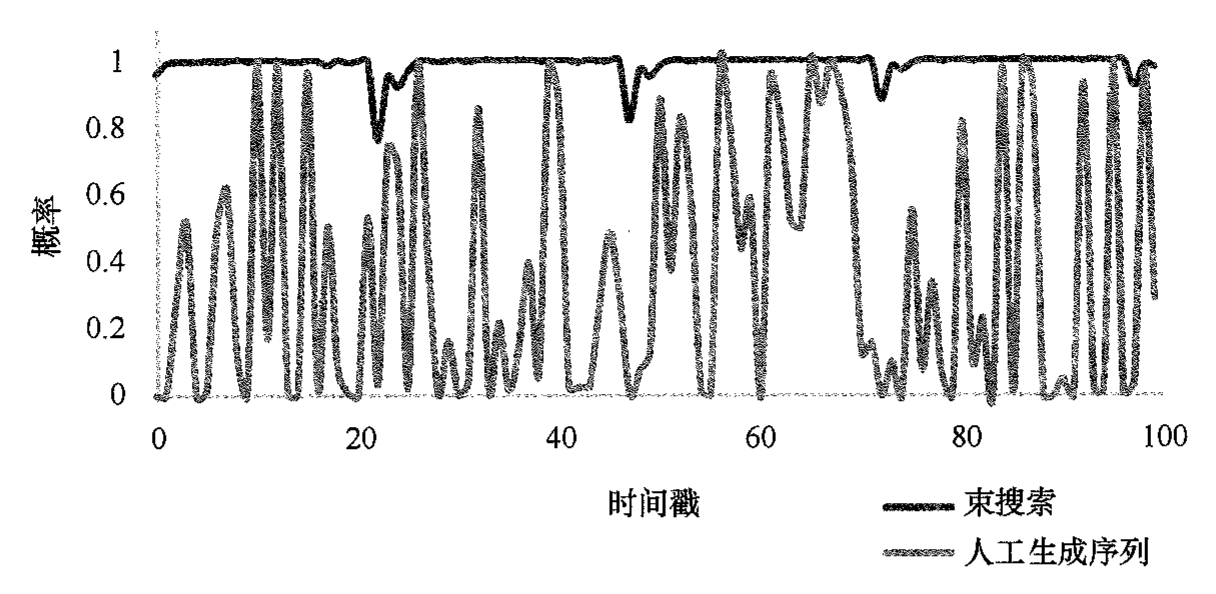
\includegraphics[width=0.85\textwidth]{ch12-fig12-17-beam-search.png}
  \caption{在给定经训练 Transformer 语言模型和初始输入序列的情况下，比较束搜索和人工生成序列的 token 概率，得出人工生成序列的 token 概率要低得多[经 Holtzman 等人（2019）授权使用]。}
  \label{figure:ch12-束搜索}
\end{figure}

我们可以在每一步从 softmax 分布中采样，生成连续的 token，而不是试图找到概率最高的序列。然而，这可能导致无意义的序列。这是因为 token 字典通常非常庞大，其中有许多 token 状态组成的长尾，每个状态的概率都非常小，但总体上却占总概率的很大一部分。这就导致一个问题，即系统很有可能对下一个 token 做出错误的选择。

为了在这两个极端之间取得平衡，对于 $K$ 的某个选择，我们可以只考虑前 $K$ 个概率的状态，然后根据它们的重归一化概率对其进行采样，称为 top-K 采样。这种方法的一个变体叫作 top-$p$ 采样或核采样（nuclear sampling），用于计算最高输出的累积概率，直至达到一个阈值，然后从这个受限的 token 状态集中采样。

top-$K$ 采样的一个“更软”版本是在 softmax 函数的定义中引入一个称为温度的参数 $T$（Hinton, Vinyals, and Dean, 2015），从而
\begin{align}
y_i=\frac{\exp\left(a_i/T\right)}{\sum_j\exp\left(a_j/T\right)}
\label{align:ch12-温度softmax}
\end{align}

\begin{definition}[温度采样]\label{definition:ch12-温度采样}
设 logits 为 $a_1,\cdots,a_K$。若按\eqref{align:ch12-温度softmax}把 softmax 的输出 $y_i$ 作为第 $i$ 个 token 的采样概率，则称参数 $T>0$ 为\textbf{温度}，相应过程称为\textbf{温度采样}。
\end{definition}

% SUPPLEMENT: parent=definition:ch12-温度采样; kind=motivation; location=紧随其后的 remark（重构新增）
\begin{remark}（重构新增）
温度把“确定性”与“随机性”放进同一个连续参数里：$T$ 越小，logits 的差异被放大，分布越尖锐；$T$ 越大，差异被压平，分布越均匀。$T=1$ 时恢复原始 softmax，因此它不改变模型的训练，只改变推理时的采样行为。它的实际作用是对长尾的抑制程度可调：$T<1$ 时低概率 token 的采样机会急剧下降，$T>1$ 时则会引入更多罕见词。注意定义要求 $T>0$：$T=0$ 时公式无定义，应理解为极限，而不是直接代入。温度采样与 top-$K$、top-$p$ 并不冲突，实际系统常先截断再调温。
\end{remark}

\begin{proposition}[温度的极限行为]\label{proposition:ch12-温度极限}
设 $a_1,\cdots,a_K$ 中最大值唯一，记为 $a_{i^*}$，$y_i(T)$ 由\eqref{align:ch12-温度softmax}给出。则当 $T\to0^{+}$ 时 $y_{i^*}(T)\to1$ 而对 $i\neq i^*$ 有 $y_i(T)\to0$，即贪婪选择；当 $T\to\infty$ 时 $y_i(T)\to1/K$，即均匀分布；当 $T=1$ 时 $y_i$ 为原始 softmax 输出。
\end{proposition}

\begin{proof}
写 $y_i=\exp\left((a_i-a_{i^*})/T\right)\big/\sum_j\exp\left((a_j-a_{i^*})/T\right)$。对 $i\neq i^*$ 有 $a_i-a_{i^*}<0$，当 $T\to0^{+}$ 时该指数趋于 $0$；分子与分母中 $i^*$ 项均趋于 $1$，故 $y_{i^*}\to1$，其余趋于 $0$。当 $T\to\infty$ 时所有 $(a_i-a_{i^*})/T\to0$，故 $y_i\to1/K$。$T=1$ 时\eqref{align:ch12-温度softmax}就是 softmax 的定义。
\end{proof}

% SUPPLEMENT: parent=proposition:ch12-温度极限; kind=motivation; location=紧随其后的 remark（重构新增）
\begin{remark}（重构新增）
该命题说明贪婪搜索不是独立于采样之外的算法，而是温度采样在 $T\to0$ 时的极限，这解释了为什么 $T$ 很小时生成文本接近确定、重复率高，而 $T$ 很大时言辞紊乱：分布被拉平后，长尾 token 与合理 token 的概率差距消失。$T\to\infty$ 的均匀极限给出了最坏情形的参照：此时模型输出与输入完全无关，退化为随机打字。这两个极限也提示调温的合理区间是 $0<T\leqslant1$ 附近。
\end{remark}

然后从修正过的分布中采样下一个 token。当 $T=0$ 时，概率质量（probability mass）集中在最可能的状态上，其他状态的概率为零，因此这就变成了贪婪挑选。当 $T=1$ 时，我们恢复未经修正的 softmax 分布；当 $T\to\infty$ 时，分布在所有状态下变得均匀。在 $0<T<1$ 的范围内选择一个值，概率就会向高值集中。

序列生成面临的一个挑战是，在学习阶段，模型是在人工生成的输入序列上进行训练的；而在生成运行阶段，输入序列本身就是由模型生成的。这意味着模型可能会偏离我们在训练过程中看到的序列分布。

\subsection{编码器型 Transformer}\label{subsection:ch12-编码器型Transformer}

接下来，我们将考虑基于编码器的 Transformer 语言模型，这种模型将序列作为输入，并生成长度固定的向量（如 $\langle\mathrm{class}\rangle$ 标签）作为输出。作为这种模型的典型代表，BERT（Bidirectional Encoder Representations from Transformers）（Devlin et al., 2018）旨在利用大规模文本语料预先训练语言模型，然后利用迁移学习（transfer learning）对模型进行微调，以完成各种下游任务，其中每种任务都需要较小的特定应用训练集。模型架构如\cref{figure:ch12-编码器BERT}所示。这种方法是前面所讲的 Transformer 层的简单应用（参见\cref{subsection:ch12-Transformer层}）。

\begin{figure}[htbp]
  \centering
  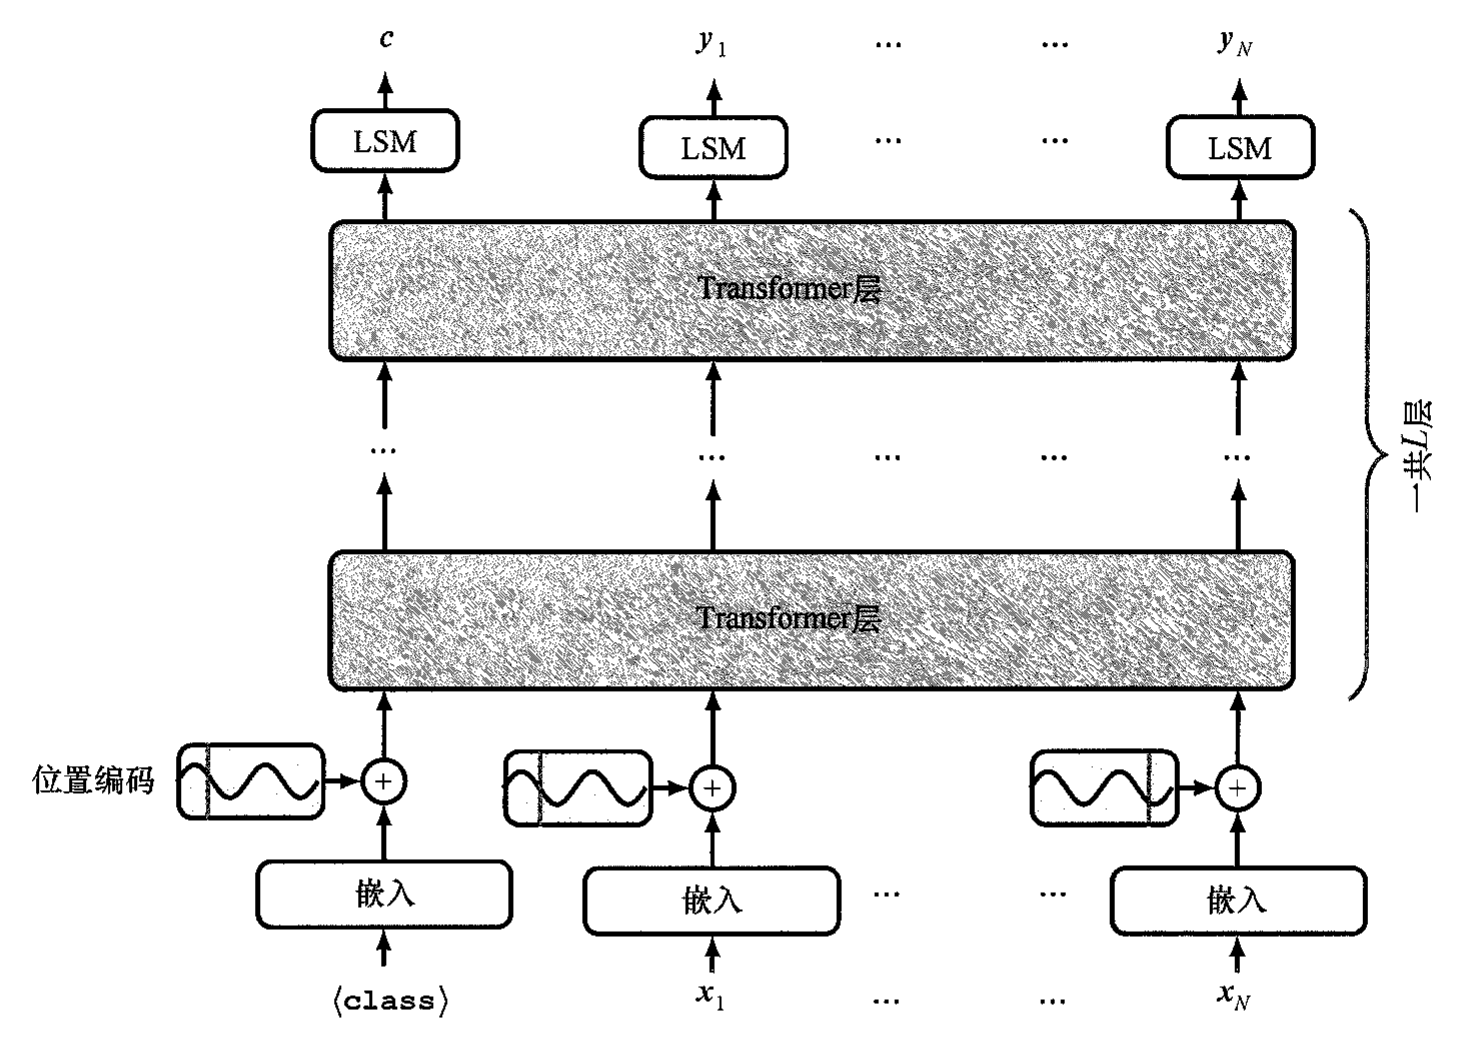
\includegraphics[width=0.8\textwidth]{ch12-fig12-18-encoder-bert.png}
  \caption{GPT 编码器型 Transformer 网络的架构。标有“LSM”的方框表示线性变换，其可学习参数在 token 位置之间是共享的，然后是一个 softmax 激活函数。与\cref{figure:ch12-解码器GPT}相比，主要区别在于输入序列没有向右移动，且省略了遮掩矩阵。因此，在每个自注意力层中，每个输出 token 都可以关注任何输入 token。}
  \label{figure:ch12-编码器BERT}
\end{figure}

每个输入字符串的第一个 token 由一个特殊的 token $\langle\mathrm{class}\rangle$ 给出，模型的相应输出在预训练时则被忽略。当我们讨论微调时，它的作用将变得显而易见。通过在输入端呈现 token 序列，可以对模型进行预训练。用一个特殊 token（用 $\langle\mathrm{mask}\rangle$ 表示）代替一个随机选择的 token 子集，比例为 15\%。该模型经过训练后，就可以预测相应输出节点上缺失的 token。这类似于 word2vec 模型中用于学习词嵌入的遮掩（参见\cref{subsection:ch12-词嵌入}）。例如，输入序列可能如下：

\begin{center}
I $\langle\mathrm{mask}\rangle$ across the river to get to the $\langle\mathrm{mask}\rangle$ bank.
\end{center}

网络应该预测输出节点 2 上的“swam”和输出节点 10 上的“other”。在这种情况下，只有两个输出有益于误差函数，其他输出则被忽略。

“双向”一词是指网络可以同时看到掩词之前和之后的词，并利用这两个信息源进行预测。因此，与解码器型 Transformer 不同的是，编码器型 Transformer 不需要将输入向右移动一位，也不需要遮掩每一层的输出，以免看到序列中后续出现的输入 token。与解码器模型相比，编码器模型的效率较低，因为只有一部分序列 token 用作训练标签。此外，编码器模型无法生成序列。

用 $\langle\mathrm{mask}\rangle$ 替换随机选择 token 的过程意味着与后续的微调集相比，训练集存在不匹配的问题，因为后者不包含任何 $\langle\mathrm{mask}\rangle$ token。为了减少这种情况可能导致的问题，Devlin et al.（2018）对随机选择 token 的过程稍微做了修改，从而在 15\% 的随机选择 token 中，80\% 用 $\langle\mathrm{mask}\rangle$ 代替，10\% 用词汇表中随机选取的一个词代替，10\% 将原始词保留在输入端（但仍需要在输出端对其进行正确预测）。

编码器模型经过训练后，就可以针对各种不同的任务进行微调。为此，需要构建一个新的输出层，其形式与所要解决的任务相匹配。在文本分类任务中，只使用第一个输出位置，其对应于总是出现在输入序列中第一个位置的 $\langle\mathrm{class}\rangle$ token。如果输出矩阵的维度为 $D$，那么第一个输出节点就会添加一个维度为 $D\times K$ 的参数矩阵，其中 $K$ 为类的数量，然后将其依次输入一个 $K$ 维的 softmax 函数或一个维度为 $D\times1$ 的向量，$K=2$ 时则将其输入一个逻辑斯谛 sigmoid 函数。线性输出变换也可以用更复杂的可微分模型（如多层感知机）替代。如果希望对输入字符串中的每个 token 进行分类，例如将每个 token 归入一个类（如人、地点、颜色等），那么第一个输出将被忽略，随后的输出会有一个共享的“线性变换 + softmax”层。在微调过程中，包括新输出矩阵在内的所有模型参数都是通过随机梯度下降法并利用正确标签的对数概率来学习的。另外，预训练模型的输出也可输入复杂的生成式深度学习模型，用于文本到图像合成等应用（参见\cref{chapter:ch20-扩散模型}）。

\begin{proposition}[掩码语言建模的损失覆盖]\label{proposition:ch12-掩码损失}
设输入序列长度为 $N$，被选中遮掩的位置集合为 $\mathcal{M}$。若只对被选中位置的输出计算交叉熵，则训练损失为 $-\sum_{n\in\mathcal{M}}\ln p\left(x_n\mid\tilde{\mathbf{x}}\right)$，其中 $\tilde{\mathbf{x}}$ 为遮掩后的输入；若 $\mathcal{M}$ 以独立概率 $q$ 选取每个位置，则每个位置进入损失的期望次数为 $q$，因而同样数目的梯度步所覆盖的“监督信号”约为自回归模型的一小部分。
\end{proposition}

\begin{proof}
损失是各被选中位置负对数似然之和，只有这些位置的目标已知，其余位置的输出不进入损失。由期望的线性性，位置 $n$ 被选中的概率为 $q$，故它进入损失的期望次数为 $q$；$N$ 个位置合计为 $qN$ 个有效标签，而自回归模型在同一序列上有 $N$ 个标签。文中取 $q=15\%$，即得结论。
\end{proof}

% SUPPLEMENT: parent=proposition:ch12-掩码损失; kind=motivation; location=紧随其后的 remark（重构新增）
\begin{remark}（重构新增）
该命题给出文中“编码器模型效率较低”的定量解释：同一段文本，自回归训练能提供 $N$ 个监督信号（每个位置都预测下一个 token），而掩码训练只提供约 $qN=0.15N$ 个。这也是编码器模型无法直接用于生成的原因——它从未学习“给定前缀续写”的条件分布。80/10/10 的替换规则则是为了缓解训练与微调的不匹配：若永远只用 $\langle\mathrm{mask}\rangle$，模型将只学会“看到 mask 就填词”，而微调时输入中根本没有 mask；保留 10\% 原词、10\% 随机词，使模型对“输入可能被污染”具有鲁棒性。
\end{remark}

\subsection{序列到序列 Transformer}\label{subsection:ch12-序列到序列Transformer}

为完整起见，我们简要讨论一下第三类 Transformer 模型，此类 Transformer 模型将编码器与解码器做了结合，正如 Vaswani et al.（2017）在最初的 Transformer 论文中所讨论的那样。请参阅将句子从英语翻译成荷兰语的任务。如前所述，我们可以使用解码器型 Transformer 逐个生成与荷兰语输出相对应的 token 序列（参见\cref{subsection:ch12-解码器型Transformer}）。主要区别在于，该输出需要以与英文句子相对应的整个输入序列为条件。编码器型 Transformer 可用于将输入 token 序列映射为合适的内部表示，我们用 $\mathbf{Z}$ 表示。为了将 $\mathbf{Z}$ 纳入输出序列的生成过程，我们使用了一种经过修正的注意力机制，称为交叉注意力（cross attention）。交叉注意力与自注意力相似，只是虽然查询向量来自正在生成的序列（在本例中指的是荷兰语输出序列），但键向量和值向量来自 $\mathbf{Z}$ 所代表的序列，如\cref{figure:ch12-交叉注意力}所示。回到我们对视频流服务的类比，这就好比用户将其查询向量发送给不同的流媒体公司，流媒体公司会将其与自己的键向量集作比较，以找到最佳匹配，然后以电影的形式返回相关的值向量。将编码器和解码器组件结合起来，即得到\cref{figure:ch12-序列到序列}所示的模型架构。该模型可以使用成对的输入句子和输出句子进行训练。

\begin{definition}[交叉注意力]\label{definition:ch12-交叉注意力}
设编码器输出为 $\mathbf{Z}\in\mathbb{R}^{N'\times D}$，解码器当前层的表示为 $\mathbf{X}\in\mathbb{R}^{N\times D}$。若查询由解码器一侧给出而键、值由编码器一侧给出，即
\begin{align}
\mathbf{Q}=\mathbf{X}\mathbf{W}^{(q)},\qquad
\mathbf{K}=\mathbf{Z}\mathbf{W}^{(k)},\qquad
\mathbf{V}=\mathbf{Z}\mathbf{W}^{(v)},
\label{align:ch12-交叉注意力}
\end{align}
再按\eqref{align:ch12-缩放点积注意力}计算输出，则称该注意力为\textbf{交叉注意力}（cross attention）。
\end{definition}

% SUPPLEMENT: parent=definition:ch12-交叉注意力; kind=motivation; location=紧随其后的 remark（重构新增）
\begin{remark}（重构新增）
交叉注意力与自注意力的唯一差别在于 $(\mathbf{Q},\mathbf{K},\mathbf{V})$ 的来源：自注意力三者同源，故 $N\times N$ 的注意力矩阵刻画“序列内部各位置的关系”；交叉注意力中 $\mathbf{Q}$ 来自解码器（长度 $N$）、$\mathbf{K},\mathbf{V}$ 来自编码器（长度 $N'$），注意力矩阵为 $N\times N'$，刻画“输出每个位置应读取输入的哪些部分”。这正是机器翻译中“对齐”的软实现：生成第 $n$ 个荷兰语词时，模型可以按权重读取英语句子的任意位置。条件 $D_q=D_k$ 仍然必要，但两侧序列长度可以不同，这也是它与自注意力在形状上最显著的区别。编码器只计算一次 $\mathbf{Z}$，所有解码层复用它，因此交叉注意力不增加编码成本。
\end{remark}

\begin{figure}[htbp]
  \centering
  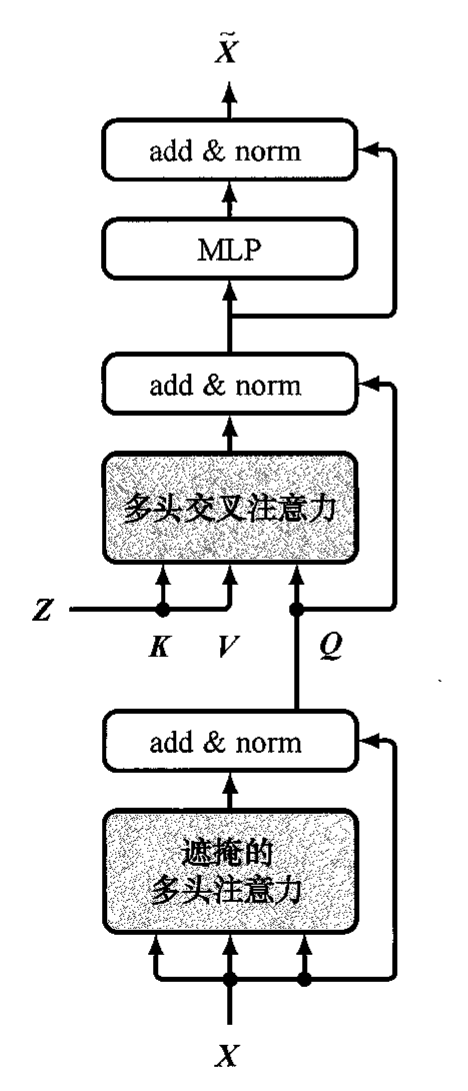
\includegraphics[width=0.42\textwidth]{ch12-fig12-19-cross-attention.png}
  \caption{序列到序列 Transformer 的解码器部分使用的交叉注意力层示意图。此处 $\mathbf{Z}$ 表示编码器部分的输出，“add \& norm”代表残差连接和随后的层归一化，“MLP”代表多层感知机。$\mathbf{Z}$ 还表示交叉注意力层的键向量和值向量，而查询向量则由解码器部分决定。}
  \label{figure:ch12-交叉注意力}
\end{figure}

\begin{figure}[htbp]
  \centering
  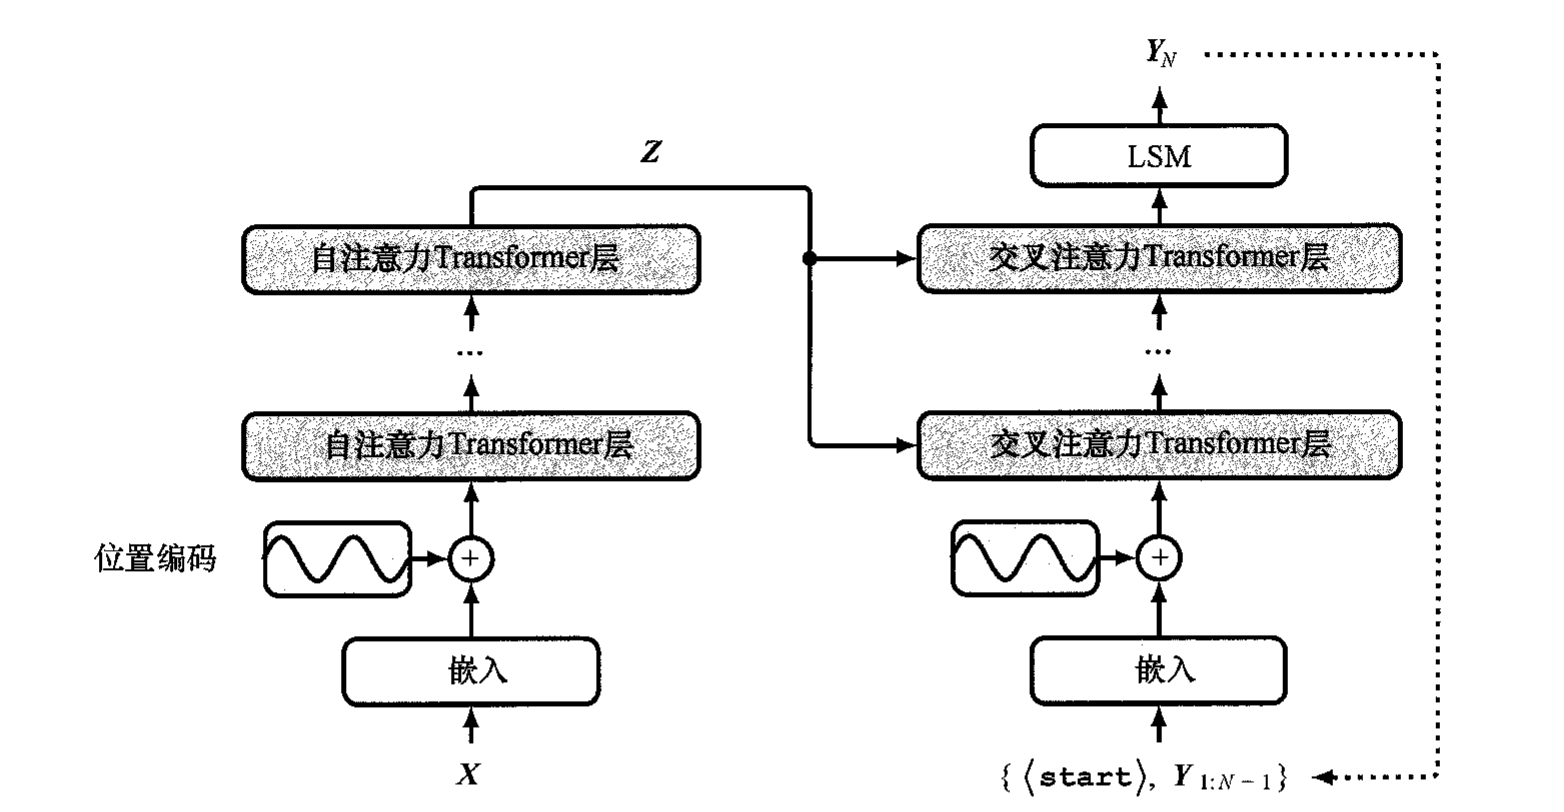
\includegraphics[width=0.9\textwidth]{ch12-fig12-20-seq2seq.png}
  \caption{序列到序列 Transformer 的示意图。在这里，输入 token 和输出 token 都显示为方框。位置编码向量被添加到编码器和解码器部分的输入 token 中。编码器中的每一层都与\cref{figure:ch12-Transformer层架构}所示的结构相对应，每个交叉注意层的形式如\cref{figure:ch12-交叉注意力}所示。}
  \label{figure:ch12-序列到序列}
\end{figure}

\subsection{大语言模型}\label{subsection:ch12-大语言模型}

机器学习领域最近最重要的发展是为自然语言处理创建了基于 Transformer 的超大型神经网络——大语言模型（Large Language Model, LLM）。此处的“大”指的是网络中权重和偏置参数的数量规模大，在撰写本书时，这些参数的数量可高达约一万亿（$10^{12}$）。这种模型的训练成本很高，但其所拥有的卓越能力促使着人们建立这种模型。

除了大型数据集的可用性，基于图形处理单元和类似处理器的大规模并行训练硬件的出现也为训练更大型的模型提供了便利，这些硬件在配备了快速互联机制和大量内置存储器的大型集群中紧密耦合。Transformer 架构在这些模型的开发过程中发挥了关键作用，因为它能够非常有效地利用这些硬件。通常情况下，增加训练集的规模，同时相应增加模型参数的数量，所带来的性能改进会超过架构改进或纳入更多领域知识的方法（Sutton, 2019; Kaplan et al., 2020）。例如，GPT 系列模型（Radford et al., 2019; Brown et al., 2020; OpenAI, 2023）连续几代性能的显著提升主要归功于参数规模的扩大。这类性能改进推动了一种新摩尔定律的产生：自 2012 年以来，训练一个最先进的机器学习模型所需的计算运算次数呈指数增长，倍增的时间约为 3.4 个月（参见\cref{chapter:ch01-深度学习革命}）。此外，这类模型的性能也在以惊人的速度不断提高。

早期的语言模型采用监督学习的方法进行训练。例如，为了建立一个翻译系统，训练集将由两种语言的配对句子组成。然而，监督学习的一个主要局限是，数据通常必须经过人工整理，以提供有标签数据，这严重限制了可用数据的数量，因此需要大量使用归纳偏置，如特征工程和架构约束，以实现合理的性能。

相反，大语言模型是通过对超大型文本数据集进行自监督学习来训练的，同时还可能包括计算机代码等其他 token 序列。我们已经了解了如何在 token 序列上训练解码器型 Transformer（参见\cref{subsection:ch12-解码器型Transformer}），其中每个 token 都是一个有标签的目标示例，而前面的序列则是输入，从而学习条件概率分布。这种“自标签”大大增加了可用的训练数据量，因而可以利用具有大量参数的深度神经网络。

使用自监督学习引发了一种范式转变，即首先使用无标签数据对一个大的模型进行预训练（pre-trained），然后使用基于小得多的有标签数据集的监督学习对模型进行微调（fine-tuned）。这实际上是一种迁移学习，同一个预训练模型可用于多个“下游”应用。具有广泛功能且随后可以针对特定任务进行微调的模型称作基础模型（foundation model）（Bommasani et al., 2021）。

我们可以通过在网络输出中增加额外层，或用新参数替换最后几层，然后使用有标签数据训练最后几层来实现微调。在微调阶段，主模型中的权重和偏置既可以保持不变，也可以进行小幅调整。与预训练相比，微调的成本通常较低。

一种非常有效的微调方法叫作低秩自适应（Low-Rank Adaptation, LoRA）（Hu et al., 2021）。这种方法的灵感来自一些结果，这些结果表明，经过训练的过度参数化模型在微调方面具有较低的内在维度，这意味着微调过程中模型参数的变化位于一个流形（manifold）上，该流形的维度远远小于模型中可学习参数的总数（Aghajanyan, Zettlemoyer, and Gupta, 2020）。低秩自适应利用了这一点，做法是冻结原始模型的权重，并以低秩乘积的形式在 Transformer 的每一层添加额外的可学习权重矩阵。通常只修改注意力层的权重，多层感知机层的权重则保持不变。考虑一个维度为 $D\times D$ 的权重矩阵 $\mathbf{W}_0$，它可能代表一个查询矩阵、键矩阵或值矩阵，其中来自多个注意力头的矩阵则视为一个单独的矩阵。如\cref{figure:ch12-LoRA}所示，我们引入了一个平行权重集，它由两个矩阵 $\mathbf{A}$ 和 $\mathbf{B}$ 的乘积定义，这两个矩阵的维度分别为 $D\times R$ 和 $R\times D$。然后，该层产生一个由 $\mathbf{X}\mathbf{W}_0+\mathbf{X}\mathbf{A}\mathbf{B}$ 给出的输出矩阵。与原始权重矩阵 $\mathbf{W}_0$ 中的 $D^{2}$ 个参数相比，附加权重矩阵 $\mathbf{A}\mathbf{B}$ 中的参数数量为 $2RD$。因此，如果 $R\ll D$，则微调过程中需要调整的参数数量远少于原始 Transformer 中的参数数量。实际上，这可以将需要训练的参数数量减少到原来的万分之一。一旦完成微调，就可以将附加权重添加到原始权重矩阵中，从而得到新的权重矩阵：
\begin{align}
\tilde{\mathbf{W}}=\mathbf{W}_0+\mathbf{A}\mathbf{B}
\label{align:ch12-LoRA}
\end{align}

在推理过程中，与运行原始模型相比，我们不会有额外的计算开销，因为更新后的模型与原始模型大小相同。

\begin{figure}[htbp]
  \centering
  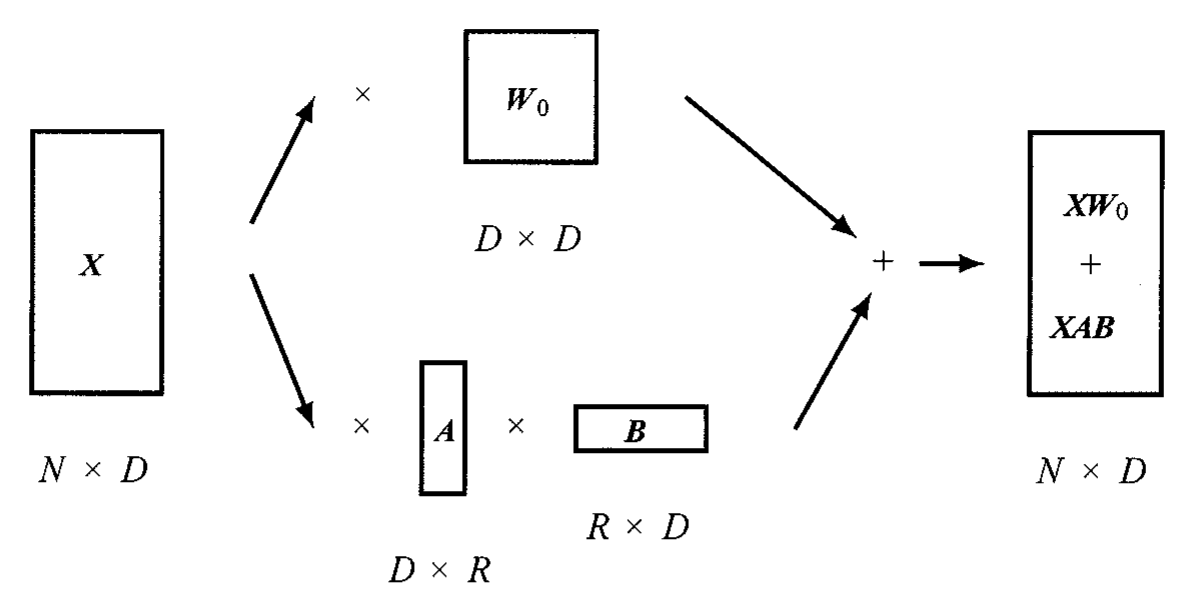
\includegraphics[width=0.8\textwidth]{ch12-fig12-21-lora.png}
  \caption{低秩自适应的示意图，这里展示了预训练 Transformer 中一个注意力层的权重矩阵 $\mathbf{W}_0$。在微调过程中，对矩阵 $\mathbf{A}$ 和 $\mathbf{B}$ 给出的附加权重进行调整，然后将它们的乘积 $\mathbf{A}\mathbf{B}$ 添加到原始权重矩阵中，用于后续推理。}
  \label{figure:ch12-LoRA}
\end{figure}

随着语言模型变得越来越大，对微调的需求越来越少，现在只需要通过基于文本的交互，生成式语言模型就能执行广泛的任务。例如，假设给出一个文本串

\begin{center}
English: the cat sat on the mat. French:
\end{center}

作为输入序列，自回归语言模型就可以继续生成后续 token，直至生成 $\langle\mathrm{stop}\rangle$ token，其中新生成的 token 代表法语翻译。请注意，该模型并不是专门为翻译而训练的，而是在包括多种语言在内的大量数据语料上训练出来的。

用户可以使用自然语言与这些模型交互。为了改善用户体验和所生成输出的质量，研究人员使用基于人类反馈的强化学习（Reinforcement Learning from Human Feedback RLHF）等方法，开发出了一些通过人工评估生成输出来微调大语言模型的技术（Christiano et al., 2017）。这些技术支持创建具有简单易用对话界面的大语言模型，其中最著名的是 OpenAI 的 ChatGPT。

用户给出的输入 token 序列称为提示（prompt）。例如，它可能包含一个故事的开场白，而模型需要完成这个故事。它也可能包含一个问题，而模型应该提供答案。通过使用不同的提示，同一个经训练的神经网络可以完成多种任务，例如根据简单的文本请求生成计算机代码，或根据要求写出押韵的诗歌。模型的性能取决于提示的形式，这催生了一个叫作提示工程（prompt engineering）的新领域（Liu et al., 2021），其目的是为提示设计一种好的形式，从而为下游任务带来高质量的输出。在将用户提示输入语言模型之前，还可以通过调整用户提示来修改模型的行为，即在用户提示前预置一个称为前缀提示（prefix prompt）的额外 token 序列以修改输出的形式。例如，前缀提示可能包括用标准英语表达的指令，以告诉网络不要在输出中包含攻击性语言。

这样，只需要在提示中提供一些示例，模型就能解决新任务，而无须调整模型参数。这是小样本学习（few-shot learning）的一个示例。

目前最先进的模型（如 GPT-4）已经变得十分强大，以至于它们表现出一些非凡的特性，这些特性被描述为通用人工智能的初步迹象（Bubeck et al., 2023），并正在推动新一轮的技术创新。

\end{document}
